\chapter{Background \& Objectives}

%This section should discuss your preparation for the project, including background reading, your analysis of the problem and the process or method you have followed to help structure your work.  It is likely that you will reuse part of your outline project specification, but at this point in the project you should have more to talk about. 
%
%\textbf{Note}: 
%
%\begin{itemize}
%   \item All of the sections and text in this example are for illustration purposes. The main Chapters are a good starting point, but the content and actual sections that you include are likely to be different.
%   
%   \item Look at the document on the Structure of the Final Report for additional guidance. 
%   
%\end {itemize}
%
%\section{Background}
%What was your background preparation for the project? What similar systems or research techniques did you assess? What was your motivation and interest in this project? 
%
%\section{Analysis}
%Taking into account the problem and what you learned from the background work, what was your analysis of the problem? How did your analysis help to decompose the problem into the main tasks that you would undertake? Were there alternative approaches? Why did you choose one approach compared to the alternatives? 
%
%There should be a clear statement of the research questions, which you will evaluate at the end of the work. 
%
%In most cases, the agreed objectives or requirements will be the result of a compromise between what would ideally have been produced and what was felt to be possible in the time available. A discussion of the process of arriving at the final list is usually appropriate.
%
%\section{Research Method}
%You need to describe briefly the life cycle model or research method that you used. You do not need to write about all of the different process models that you are aware of. Focus on the process model or research method that you have used. It is possible that you needed to adapt an existing method to suit your project; clearly identify what you used and how you adapted it for your needs.

\section{Background}

\subsection{Introduction}

%As human beings, we are expected to make decisions both large and small as part of everyday life. While the act of making a decision is constitutes an action that is rarely consciously observed, others that may have potentially life-changing consequences will force an individual to consider much more closely.
%
%For a human faced with making such decisions, identifying which out of a number of possible choices constitutes the ``right" decision is often regarded as a challenging and highly subjective task. %Each decision that a person makes will vary based upon their individual characteristics, which as a consequence can often result in contrasting decisions being taken in response to the same situation.% 
%Before settling on a final decision, an individual will typically identify and evaluate all possible choices by considering each upon a weighting of merit \cite{rational-decision-model}. While variations in weighting between specific individuals can cause different decision outcomes, an important realisation comes from the understanding that all considerations made by an individual rely on their \textit{trust} in the accuracy and truth of information gathered during the identification and comparison of these alternative choices.

 In considering any kind of autonomous system that is expected to make unattended decisions, a crucial, yet not always obvious aspect is a reliance upon the idea of \textit{trust}. As is observed in humans, such a system will typically depend upon underlying information in order to assess which, out of a selection of alternative choices, is the most appropriate for a given situation.
 
 This information may be obtained from a variety of sources, ranging from raw sensor data up to the output of a sophisticated algorithm. While the type and source of information may vary wildly between systems, the underlying notion that this information can, in one form or another, be \textit{trusted} to provide a truthful representation of the current situation remains the same. 
 
Given the importance of the relationship between reliable input data and correct decision making, a crucial aspect associated with autonomous robotics is the attempt to maximise both accuracy of input data, and robustness of systems used to verify this accuracy.

  The ability to navigate plays a vital role in enabling robots that require autonomous motion capabilities to make safe, yet objective decisions on how best to traverse from one position to another. This becomes evermore important when considering that a key use case for robotic systems typically involves the undertaking of tasks within environments deemed unsafe for humans to enter. From observing examples of tasks where autonomous robots are expected to operate within harsh environments including bomb disposal and planetary exploration \cite{maimone2007two}, it becomes clear that the ability to perform safe and robust navigation is vital to the survival of both the mission and device.

%As a problem-space, autonomous navigation can be decomposed into two key areas of focus; one of \textit{reactive} navigation, and the other of \textit{deliberative} navigation. Reactive, or local navigation is concerned with controlling the path of the robot through the immediate surrounding area, focussing in particular on the safe traversal around potentially dangerous terrain hazards including obstacles, steep slopes and precipices. In contrast, deliberative or global navigation is tasked with planning the ``high-level" path that a robot will follow in order to reach its destination. As a consequence, deliberative navigation tends to adopt a greater level of focus on calculating the most \textit{optimal} path through the environment over necessarily the one that is ``safest" for the robot. Traditionally within autonomous navigation systems, feedback from both the reactive and deliberative components is combined in order to arrive at final path that balances both safety and objectivity \cite{mer-rover}. 

A vital contributor to enabling successful navigation, is the ability to identify and subsequently avoid obstacles. As such, the development of accurate and robust obstacle detection systems is a keen and well-explored area of robotics research, with a variety of approaches now available adopting many types of sensor including sonar \cite{williamson} and laser scanning \cite{wyeth}. 

An alternative approach that has enjoyed increasingly greater research focus over the past decade is that of vision-based obstacle avoidance. This involves the analysis of images captured from one or more digital cameras in order to detect and classify possible dangers situated within the robot's field of view. 

Cameras are becoming an increasingly favourable sensor for use on robotic systems, due primarily to the impressive variety and quantity of potential data that can be captured \textit{simultaneously} from a single device. They are also one of few sensors that have experienced a consistent reduction in price over the past decade \cite{campbell}, making them viable for many types of project application and budget. 

\subsection{Related Work}
\label{related-work}

The challenge of providing accurate and robust obstacle detection remains to be a major topic of focus within the field of computer vision. While beginning to investigate this area of research, it quickly becomes clear that there are an enormous variety of solutions already available. In the majority of cases, these solutions propose new or improved approaches to combining ``standard" computer-vision techniques with a variety of hardware configurations, with the aim of either improving on previously published results, or to focus on the avoidance of specific types of obstacle (e.g. precipice or animal detection). 

%From investigating existing research conducted in the area of visual-based navigation and obstacle avoidance, it is possible to identify and compare potential benefits and challenges between various approaches that will in turn feed into future design decisions.

%\subsubsection{Feature-Based Methods}

The first approach to be noted is that from the work of Campbell \textit{et al} \cite{campbell}, in which the authors propose a system for estimating the change in position and rotation of a robot using information obtained solely using a single consumer-grade colour camera. The approach describes the use of feature-based tracking to estimate the sparse optical flow-field between subsequent video frames, before taking these optical flow vectors currently corresponding to image coordinates, and back-projecting them onto a ``robot-centred" coordinate system in order to establish the incremental `real world' translation and rotation of the robot over a given time period. The detection and subsequent tracking of matching features between captured frames is provided via the \textit{OpenCV} library implementation of the Lucas-Kanade algorithm \cite{shi1994good}. 

%Once gathered, these correspondences between features (i.e. optical flow vectors) are filtered to help remove outliers caused by matching error or occlusion. The criteria used for this filtering process focusses on verifying a smooth straight-line motion of same features between subsequent frames. It is reported that concentrating on the movement history of features across a subset of previous frames can provide a robust defence against outliers. This is because by definition, an outlier would typically be expected to be found outside of the projected straight-line trajectory of the mis-matched feature, thereby causing the motion behaviour of this feature to suddenly become erratic. Through the use of this filtering technique in conjunction with the correction of perspective distortion via calibration, the authors report they are able to allow for a wider, and potentially lower quality range of features to be initially detected in order to ensure adequate coverage of the entire image scene. 
%
%In the final stage of the process, the current frame is sectioned into regions representing the ``sky" and ``ground" individually, from within which the observed optical flow vectors are used to calculate an estimation of the robot's incremental rotation and translation respectively.

%The authors report that this implementation provides a more efficient and robust version of the original algorithm proposed by Lucas and Kanade \cite{lucas-kanade-features}. Upon further investigation this improvement appears to be attributed to the proposal published by Bouguet \cite{j-bouguet} in which the author combines a multi-scale pyramidal representation of an image with the existing Lucas-Kanade algorithm. This approach can help to provide both greater accuracy, by locating features that may have moved distances greater than the current window size, while also improving efficiency by means of reducing the size of the search area within higher resolution versions of an image, by first localising the general target area within lower resolution versions that are less computationally expensive to search. 

Of particular interest from the work of Campbell \textit{et al} \cite{campbell} is the approach described for detecting environment hazards solely via the exploitation of the optical flow field. The proposed method bases itself around the observed discontinuities caused to the optical flow field by scene objects that appear at a different observed depth to camera than the ground. In the paper this behaviour is described as a violation of the ``planar world hypothesis" \cite{campbell}, in which objects appearing closer to the camera relative to the ground cause a positive violation, and in the opposite case causing a negative violation. 

As a consequence, the authors discuss how owing to the effects of motion parallax, it is possible to observe clear differences in the motion displacement of scene objects demonstrating either a positive, negative or no violation. This subsequently maps onto discontinuities observed in the optical flow field, with objects that move significantly closer to the camera relative to the ground demonstrating longer optical flow vectors, and objects further away from the camera demonstrating the opposite. This approach appears to demonstrate notable results, with the authors describing how in practice their system was able to ``detect precipices as near as 3cm" \cite{campbell}. 

An alternative approach proposed by Low and Wyeth \cite{wyeth} involved combining sparse feature detection with appearance-based matching in order to track corresponding features between video frames. Using the template matching function provided by the \textit{OpenCV} library, the authors describe how a variety of appearance-based matching metrics could easy be evaluated via simple changes to function parameters. They report on how they eventually chose Normalised Cross-Correlation as the final similarity metric, owing primarily to its improved robustness to lighting changes and simple score range falling between 0 and 1 (1 indicating a perfect match) that allowed for easy pixel thresholding.

%This detector is almost identical to the original Harris corner detector \cite{harris-corner} from which it is based, with the only main difference focussing on a change in the use of Eigenvalues to score and classify if an image region should be identified as a corner or not. This slight modification was demonstrated by Shi and Tomasi to provide a greater level of tracking stability and robustness in comparison to the original Harris corner detector \cite{shi-tomasi-good-features-to-track}, and as a result is typically preferred over the original detector proposed by Harris and Stephens. 

%Once obtained, optical flow information was converted to more suitable range data using a method known as `Time-to-Contact'. Using this approach it is possible to represent distance to a known target as a unit of time \cite{alenya}, and is itself based heavily upon biological mechanisms identified as being responsible for providing the correct timing of actions and motion within the brain of humans and birds \cite{lee-young}. Other examples of the use of Time-to-Contact within vision-based systems providing obstacle detection include \cite{alenya}, \cite{sagrebin} and \cite{thomas}.

%Contrasting with the more ``ad-hoc" approach adopted by Campbell \textit{et al}, Low and Wyeth choose to generate a map that represents obstacle range information in order to support the detection of obstacles via the analysis of angular range output. 

A major challenge relating to the use of optical flow methods for obstacle detection, and one discussed in the work of both Low and Wyeth \cite{wyeth} and Campbell \textit{et al} \cite{campbell}, is the effect that changes in rotation (deliberate or otherwise) can have on the observed optical flow vectors of features. While both papers propose alternative methods for removing the effects of rotation (the use of an Inertial Measurement Unit gyroscope in the case of Low and Wyeth, and a calibrated cylindrical coordinate model in the case of Campbell \textit{et al}), both appear to agree that rotational movement should be accounted separately to translational movement in order to ensure accurate motion estimates can be inferred from the optical flow field. 

Ulrich and Nourbakhsh \cite{ulrich-nourbakhsh} present an alternative approach to vision-based obstacle detection from the two previously discussed. As opposed to scrutinising differences in motion behaviour of scene objects, the authors instead focus on comparing differences in colour between the ground and other objects in the robot's field of view. Ulrich and Nourbakhsh argue that using colour as a detection metric for obstacles can prove to be less computationally expensive than ``range-based" obstacle detection methods like optical flow or stereo vision, and in certain cases, have also shown to be more accurate and reliable - particularly in cases involving the detection of small or flat objects close the ground or where a system needs to be able to differentiate between terrain surfaces. 

A key aspect from the Ulrich and Nourbakhsh paper discusses details of how their system is able to effectively handle image noise caused by changes in illumination. In their solution, the authors discuss the use of an alternative colour space to RGB for representing input images that allows for the undesired effects caused by changes in illumination between subsequent frames to be negated. By converting images to use the `Hue-Saturation-Intensity' colour space, the actual colour of objects within the image (represented by the Hue and Saturation channels) become less sensitive to changes in brightness (represented by the Intensity channel). As well as providing greater resistance to illumination changes, using a colour space that separates colour from brightness also provided an easier platform from which the authors could further remove noise via channel thresholding \cite{ulrich-nourbakhsh}. 

As part of a survey conducted into various methodologies of appearance-based template matching methods, Perveen \textit{et al} \cite{perveen} discuss an enhancement to traditional template matching that has been shown to support the successful detection of objects whose observed appearance has been altered following a change in orientation. 

  The development of vision-based systems that are invariant to object rotation has been an area of keen research interest over recent years. While a number of solutions now exist for providing resilience to such changes \cite{sift}, the majority of these solutions are only applicable to detection methods that are based upon the use of feature descriptors for representing scene objects, rather than the use of an object's appearance. 
  
  This is particularly important given the assumption that for most objects, even a slight rotation will cause its \textit{appearance}, in terms of pixel values, to be modified considerably. As such, a key weakness of appearance-based detectors describes a failure to find correct matches of an object that has undergone a rotation. This is generally caused as a result of such detectors relying on an explicit pattern of object appearance for use as the primary metric when comparing image patches for similarity equality.
 
 In their paper, Perveen \textit{et al} describe how ``Grayscale-based template matching" utilises multiple pyramid structures (used traditionally in supporting degrees of scale invariance \cite{lowe}) to provide support for rotational-invariance within appearance-based features detectors. By generating a new pyramid structure to represent every possible orientation of the target pattern, these structures can, once combined, be used to significantly improve the chances of a pattern being relocated in the current image, even after potentially experiencing a significant rotational transformation \cite{perveen}. Additional work published in \cite{kim} discusses further improvements to the efficiency of this approach by removing pixels deemed unlikely to ever match a target pattern from further consideration, thereby reducing computational cost. 

%Later in the same survey, Perveen \textit{et al} discuss an additional modification to traditional template matching methods that they describe as able to exploit an important observation from object-appearance behaviour in order to provide a dramatic reduction in the computation time required for processing image patches. This observation, and the potential consequences it can pose in terms of efficiency gains, was described by the authors as:
%
%\indent \textit{``The shape of any object is defined solely by the shape of its edges. Therefore instead of matching of the whole pattern, we could extract its edges and match only the nearby pixels, thus avoiding some unnecessary computations. In common applications the achieved speed-up is usually significant."} \cite{perveen}
%
%Further investigation has shown that a number of previous robotic projects have successfully utilised edge detection as a means of providing accurate obstacle detection \cite{hanumante} and \cite{borenstein}. Also of interest was the work conducted by Lin and Chunbo \cite{lin} in which they propose a solution into the issue of rotation invariance within appearance-based detection methods through combining of the use of contour images with the ``mean absolute difference" template matching method. 

\subsubsection{Hardware Configuration}
 
While the majority of approaches mentioned thus far focus on the use of monocular-based systems (i.e a single camera) for their hardware configuration, many other examples of vision-based systems using alternative choices of hardware are also available. One of the most popular alternatives to monocular camera systems is a concept that can be easily described as `natural progression' in terms of technological evolution. This description is of course talking about the use of two or more cameras, formally known as stereo vision. 

Williamson \cite{williamson} proposes a trinocular stereo vision system capable of detecting small obstacles over great distances - \textit{``objects as small as 14cm high over ranges well in excess of 100m"}. He discusses how by using three cameras arranged in a triangular formation, his obstacle detection system is able to maintain high levels of reliability even in situations where an image demonstrates \textit{``texture in one direction, but not in the other"}. This reliability is particularly important when you consider that typical examples of this type of behaviour have been found to originate around pixels representing the edges of objects that such a system is aiming to detect \cite{williamson}. 

Williamson also later states that through the use of more than one camera, his system is able to enjoy an improved level of general accuracy, achieved as a result of the significant level of additional information that can be gathered. Taking this statement solely at face value, it could be feasible to assume that the addition of further cameras may improve on this performance further still. On a contrary to this, Williamson warns that using anymore than three cameras will not make any significant difference to performance results, and in fact may actually impede results as a consequence of over-complication \cite{williamson}.

As mentioned previously, Low and Wyeth \cite{wyeth} chose to combine the efforts of a monocular vision system, laser scanner and inertial measurement unit to provide highly accurate detection capabilities for a variety of obstacle types and sizes. A key advantage to adopting a hybridised hardware configuration comes from benefit that should one system fail for any given reason, in most circumstances, alternative systems remain available to continue. As such, multi-instrument setups can help to ensure that potentially critical information regarding the location of possible obstacles is not lost. 

However, an important consideration to note is that by increasing the variety and number of hardware components, other critical quantities relating to the design of a robot including aspects such as power usage and chassis space, may also need to revised accordingly.

%\subsection{Project Overview}
%
% 
%
%%Through this system, it should be possible to identify the presence of both positive, and negative obstacles (e.g. rocks and pits respectively), providing a reasonable indication of their general size and location. In addition, it is predicted that such a system will also be able to provide an estimation of the speed and change in orientation of the robot as it traverses along a path. These will be calculated as by-products of the terrain inference mechanism, and could be expected to eventually form part of a larger visual odometry and/or autonomous navigation system.
%
%While this project is primarily research-focussed, an ultimate goal would be to install such a system onto a working mobile robot. In particular, the `IDRIS' all-terrain four-wheel-drive autonomous robot currently owned and operated by the Department of Computer Science at Aberystwyth University.
%
%% FIGURE: IDRIS

\subsection{Motivation}

Motivation for the undertaking of this project comes following an increased interest into the field of computer vision and its associated topics, gained during completion of a university module surrounding the subject.

The project also presented a key opportunity for the author to engage in a substantial piece of work falling well outside of their prior experience, choosing to pursue a problem of a scientific or research-based nature, rather than one of `traditional' software engineering. 

Further opportunities were also presented for enhancing development skills using the C, C++ and Python programming languages, and in particular, the development of computer vision applications using popular image processing libraries.

\section{Development of the Working Hypothesis} 

Focussing on conducting research as part of a scientific investigation, this project looks specifically into investigating the viability of the following proposed hypothesis: 

\indent \textit{``From images captured using a non-calibrated monocular camera system, analysis of optical flow vectors extracted using localised appearance-based dense optical flow techniques can provide certain estimates into the current condition of terrain gradient, the location and characteristics of obstacles, and robot egomotion."}
 
In the context of this project, such a statement is technically characterised as a \textit{working hypothesis}, which gives rise to the expectation for further investigative work to be conducted, even if this hypothesis is later discovered to fail \cite{century}. 

The history of work that led to the proposal of the above hypothesis actually began focussing not on obstacle detection, nor the inference of terrain gradients, but instead on investigating potential solutions towards a lightweight visual-based odometry system for installation aboard a mobile robot. 

It was not until the completion of initial background investigations into existing approaches (namely the work of Campbell \textit{et al.} \cite{campbell} - discussed further in Section \ref{related-work}) that key ideas surrounding the final hypothesis began to come into fruition. 

\subsection{Key Aspects \& Assumptions}
\label{assumptions}

The hypothesis detailed in this report can be decomposed into four key areas of prediction. While all relate to the exploitation of observed optical flow behaviour, each focusses on providing an estimation into the status of a specific ``condition metric". 

While these will of course only be estimates, it was hoped that when brought together, these observations could provide a vital insight into the overall status and condition of the current terrain and robot egomotion. 

The four ``condition metrics" subject to observation under the proposed hypothesis were as follows:

\begin{itemize}
	\item \textbf{Terrain gradient} - Indication of how ``flat" the terrain surrounding the robot current is. Any significant changes to terrain slope (positive or negative) should be identified in order to allow any appropriate action (e.g. reduction in speed) to be taken.
	\item  \textbf{Oncoming obstacles} - The detection of both positive and negative obstacles (e.g. rocks and pits respectively) encountered along the path of a mobile robot as it moves through its environment. 
	\item \textbf{Robot speed} - Indication of a robot's speed based upon a prior knowledge of a fixed time interval and the distance moved by the robot within that time frame.
	\item \textbf{Robot orientation} - An indication of current orientation, based upon observations into changes in rotation made as a result of the robot turning. 
	
\end{itemize} 

Given the high level of potential scope for investigation presented under the working hypothesis, it was deemed important, especially in the early stages of investigation, to draw some appropriate assumptions that could help simplify the general ideas presented into manageable stages. Clearly, should the initial findings be found to be positive and enough available time remained, then it was expected that further work could be planned in order to try and tackle the more complex issues that would address these assumptions.

Taking guidance from the previous projects \cite{campbell}, \cite{wyeth}, the chosen assumptions were deemed reasonable in relation to the main objective of providing visual-based terrain inference, obstacle detection and egomotion estimation of a wheeled robot:

 \begin{enumerate}
 	\item In the first instance, it was assumed that the proposed system would only support motion following straight line trajectories. This meant that at least within the early stages of investigation, work would not focus on providing an estimation into robot orientation, given that theoretically this should not change while the robot is moving in a forward direction.
 	\item It is assumed that camera to be used as input will be mounted in fixed position facing in the same direction as the robot during forward travel.
 	
% 	An obvious exception to this was the proposed ability to estimate changes in robot orientation, which in theory would have to be caused by the robot changing direction. This however would itself make the frankly unrealistic assumption of the camera suffering no shake caused by traversal over uneven terrain. 
 \end{enumerate}

The remainder of this section is dedicated to providing details regarding the core ideas proposed within the hypothesis, including a discussion into the general thought processes considered while being conceptualised.

\subsection{Depth Estimation via Motion Parallax \& Optical Flow}

The concept of motion parallax, and its usefulness as means of inferring information about real-world environments, is an idea found to be commonplace in vision-based solutions wishing to extract details about 3D environments from 2D images \cite{lu}.  

The general theory behind motion parallax is simple, stating how as the visual field of an observer changes due to moving position, objects located a short distance away will appear to move across the scene faster than those objects located in the distance (Figure \ref{fig:parallax}). This effect forms a type of visual cue, from which the depth of objects situated within a 3-dimensional scene can subsequently be perceived \cite{rogers}.

One of the key advantages to using motion parallax within the context of computer vision is that the perceived effects continue to be visible even if captured through only a single camera. Therefore strictly speaking, motion parallax is best defined as providing a \textit{monocular} visual cue for depth, theoretically open to exploitation by any visual-based system making use of at least one camera for supplying input.

\begin{wrapfigure}{r}{0.6\textwidth}
\vspace{-20pt}
  \begin{center}
    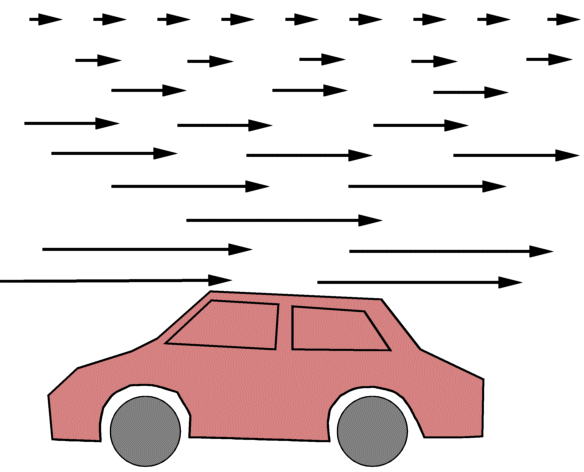
\includegraphics[width=0.5\textwidth]{images/motion_parallax.png}
  \end{center}
  \vspace{-10pt}
  \caption{Visualisation of the changes in perceived displacement of objects within the visual scene as a result of the effects caused by motion parallax. Courtesy \cite{akshay}.}
     \label{fig:parallax}
  \vspace{-20pt}
\end{wrapfigure}
 
 By measuring the level of displacement that an object demonstrates, it then becomes possible to infer the relative distance between that object and the current view position. Typical approaches within computer vision accomplish this task through the use of feature detection and tracking to subsequently calculate the displacement of static objects between consecutive images. 

In the case of Campbell \textit{et al.} \cite{campbell}, the authors make exclusive use of the observed differences in the displacement of objects as the underlying mechanism for  detecting the presence potential obstacles. 

Measuring the displacement by which a select number of ``distinctive" image regions move over time, is a process commonly known as \textit{sparse optical flow} \cite{nourani}.

 By monitoring discontinuities in the length of calculated optical flow vectors (i.e. the distance and direction of displacement along the image plane), Campbell \textit{et al.} were able to detect the presence of both positive and negative obstacles, characterised respectively by whether the features identified in the image demonstrated vectors that were proportionally \textit{shorter}, or \textit{longer} than the general consensus set \cite{campbell}.

A potentially problematic issue associated with sparse optical flow and feature detection in general, is how to ensure adequate coverage and frequency of features, when the scene represented in consecutive images fails to contain many regions ``distinctive" enough for use by feature detectors. When faced with this issue, Campbell \textit{et al.} \cite{campbell} chose to deliberately select a wider range of lower quality features within input images in order to ensure that they obtained reasonable coverage across the entire image space. 

Naturally, choosing specifically to allow the detection of lower-quality features opens up a greater risk to outliers and false positives, which Campbell and his team later counteract through the combined filtering and `peer-verification' of incremental optical flow vectors \cite{campbell}. While this approach is noted to strike a good balance between the amount of information that can be extracted and resilience to potential outliers, it does of course also attribute itself to an increase in the overall computational cost of the system. This is a price that aboard some robotic systems could prove simply to be too high, particularly in situations where spare computing power is already considered a luxury (e.g. planetary rovers). 

As alternative solution is to instead attempt to track the change in motion of \textit{every pixel} in the image, known formally as \textit{dense optical flow} \cite{nourani}. While this approach guarantees coverage across the entire image, it can also prove to be noticeably slower to complete.

\subsection{Supporting Inference of Terrain Gradient \& Obstacle Detection}
\label{hypo-gradient}

The proposed hypothesis aimed to take the same fundamental ideas proposed by Campbell \textit{et al.} \cite{campbell} for the detection of obstacles located within the visual field (discussed more in Section 
{related-work}), before attempting to apply them further to the inference of terrain gradient conditions. 

It was considered that, just in the same way as positive obstacles appear closer to the camera than the ground on which they lie, an area of ground that demonstrates a sudden increase in its tendency upwards would also conceptually appear ``closer" to the camera. 

When the resulting optical flow field is later analysed, it would be expected that the same region of the ground plane (captured over consecutive images) would demonstrate optical flow vectors that became gradually longer than those previously recorded as a result of the parallax-induced motion being observed. Likewise, when presented with an area of ground sloping evenly downwards, a decrease in its displacement detected through the observation of proportionally shorter optical flow vectors would generally be expected.  

Continuing to employ the concept of motion parallax as the primary means of estimating the 3D-geometric characteristics of a captured 2D scene, the hypothesis introduced two key differences in its general approach from those discussed within other projects investigated:

\begin{itemize}
	\item The exclusive use of appearance-based template matching techniques to provide a \textit{localised} variant of \textit{dense optical flow analysis} over the use of sparse optical flow techniques relying upon a high number of available image features.
	\item The use of a formalised model to represent detected changes in vertical displacement as part of efforts to estimate changes in terrain gradient in addition to the location/characteristics of potential obstacles. 
\end{itemize}

\subsubsection{Appearance-Based Feature Detection \& Tracking}
\label{hypo-tracking}

The decision to use appearance-based matching for the detection and subsequent tracking of features was taken primarily out of an interest in conducting an evaluation into the performance of such methods with respect to optical flow analysis. 

While examples of previous work describe the combination of feature-based detection with appearance-based tracking \cite{wyeth}, this investigation wished to focus exclusively on the use of appearance-based methods for both the initial detection, and subsequent matching/tracking of image features necessary to establish the optical flow field.

One of the key motives behind this decision directed towards the common observation that appearance-based detectors on average tended to be less computationally expensive than their feature-based equivalents \cite{wyeth}. This was an aspect that tied in closely with the relationship that the project exhibited between the fields of computer vision and robotics, and subsequently was deemed an important benefit in relation to the ultimate goal of installation aboard a mobile robot that would most likely possess limited computing capability.

In the interests of time, the project decided to focus on the evaluation of four appearance-based similarity measures for template matching identified through the background research. These consisted of two \textit{distance-based} measures, and two \textit{histogram-based} measures.

\subsubsection{Vertical Displacement Model}
\label{hypo-model}

The use of a model for representing vertical displacement of image regions was an idea that lay at the centre of the main investigation. Its purpose was to provide a mechanism by which the core underlying prediction relating to the estimation of changes in terrain gradient and obstacle detection could be evaluated:
	
	\indent \textit{``Following the concepts of motion parallax, it is predicted that features captured towards the bottom of an image will show greater displacement between subsequent frames, than those features captured towards the top of the image."}
	
The model was designed to take the form of a kind of ``lookup-table", where a simple structure would be adopted to focus specifically on the relationship between the \textit{height within an image}, and the \textit{level of vertical displacement that the row located at that height demonstrated}. 
 
 When visualised as a 2D scatter plot (Figure \ref{fig:model}), this structure definition would be represented as:
	
	\begin{itemize}
		\item \textbf{X axis:} The height of the image, plotted as 1px-high rows.
		\item \textbf{Y axis:} The vertical displacement in pixels recorded at a given height.
	\end{itemize}
	
	where the predicted trend would see as the row number (i.e. height relative to the top of the image) increased, so to would the level of vertical displacement.
	
The use of the model relies upon the completion of an initial calibration stage, in which a robot would navigate across an area of terrain that was generally considered to be both flat and clear of obstacles. During this time, a ``baseline" vertical displacement model is generated by taking an average of the displacement recorded for each image row across a number of separate measurements. 

\begin{wrapfigure}{r}{0.5\textwidth}
\vspace{-30pt}
  \begin{center}
    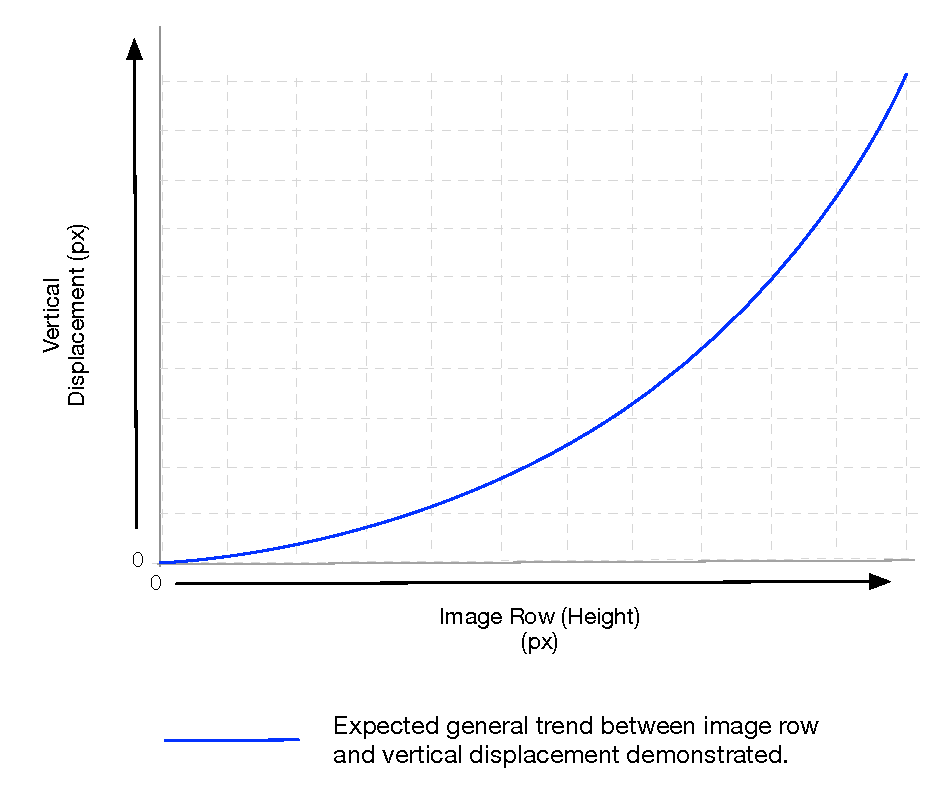
\includegraphics[width=0.5\textwidth]{images/model.pdf}
  \end{center}
  \caption{Example of a ``perfect" vertical displacement model, showing the expected positive correlation between vertical position of a patch within an image, the the level of vertical displacement demonstrated.}
  \label{fig:model}
    \vspace{-30pt}
\end{wrapfigure}
	
Within the scope of the proposed final system, subsequent comparison of displacement magnitude and direction recorded for a given row is performed against the general trend of this ``baseline" model as a means of identifying cases of ``unusual" displacement behaviour. This comparison is re-evaluated upon every system cycle, following the generation of a new model to represent the changes in the scene captured by the latest images from the camera. 

Observing a significant extension or reduction in the length of displacement recorded between the ``baseline" model and the latest version of the model would provide a strong indication to the presence of a potential obstacle (positive or negative) or change in the slope gradient of the ground (Figure \ref{fig:obstacle}).

  % ADD FIGURE SHOWING EXAMPLE OF NEGATIVE OBSTACLE AND ONE OF POSITIVE OBSTACLE.
  
 Establishing the difference between a change in displacement caused by an obstacle, and one caused by a change in terrain gradient comes down to the evaluation of the pattern of displacement recorded across all of the rows in the image.
 
 In the event of an oncoming obstacle, the rows representing that object in the image would be expected to demonstrate a significant increase (positive obstacle) or decrease (negative obstacle) in the level of displacement shown. 

\clearpage
\begin{wrapfigure}{l}{0.5\textwidth}
\vspace{-20pt}
  \begin{center}
    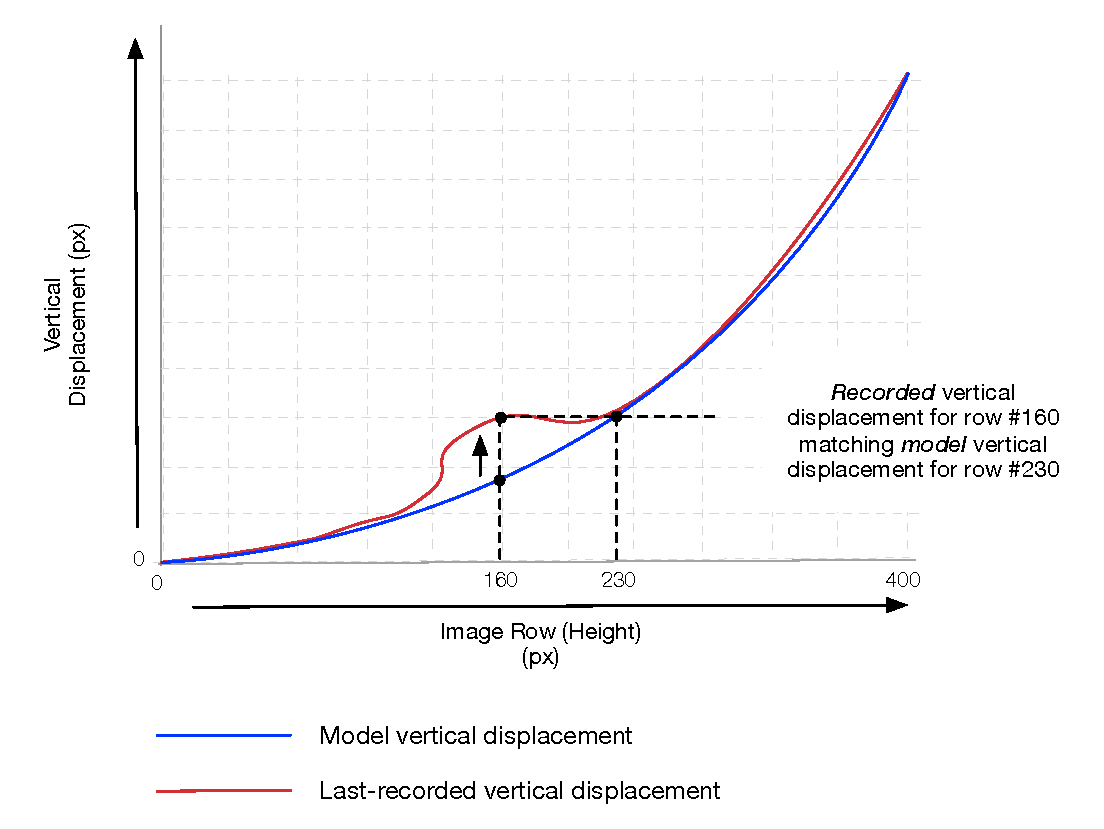
\includegraphics[width=0.49\textwidth]{images/obstacle_graph.pdf}
  \end{center}
  \vspace{-10pt}
  \caption{Example of vertical displacement model indicating the potential presence obstacle of a positive obstacle.}
  \label{fig:obstacle}
  \vspace{20pt}
\end{wrapfigure}

However importantly, this change would typically not be representative of the general trend in displacement that is observed across the entire height of image (indicated as a `spike' in a 2D scatter plot (Figure \ref{fig:multi_obstacle}). 

 Alternatively in the event of a change in terrain gradient, it would instead be expected that the vast majority of those pixels representing the ground would all demonstrate a similar change in displacement in terms of both direction and magnitude (Figure \ref{fig:gradient}). This is because a change in the slope of the actual \textit{ground} is likely to be observed across a much larger range of rows than what would be observed for an individual obstacle such as a rock or pit.

\begin{figure}[htbp]
\begin{minipage}[b]{0.5\linewidth}
\centering
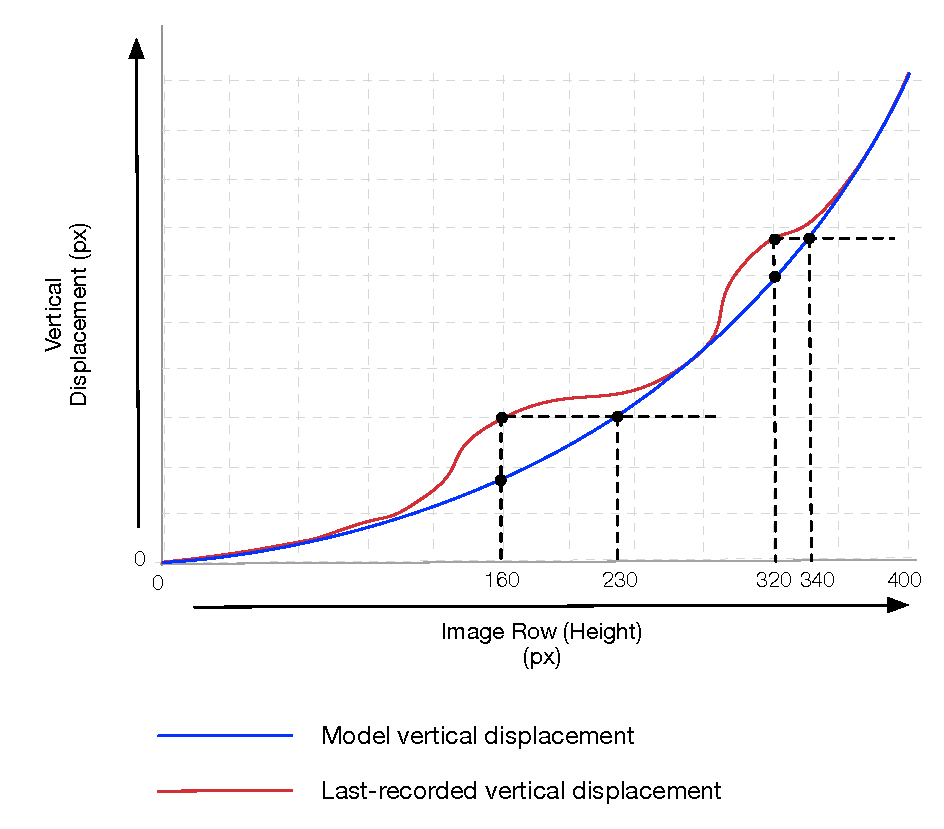
\includegraphics[width=\linewidth]{images/multi_obstacle_graph.pdf}
\caption{Simplified example of detection of multiple positive obstacles.}
\label{fig:multi_obstacle}
\end{minipage}
\hspace{0.5cm}
\begin{minipage}[b]{0.5\linewidth}
\centering
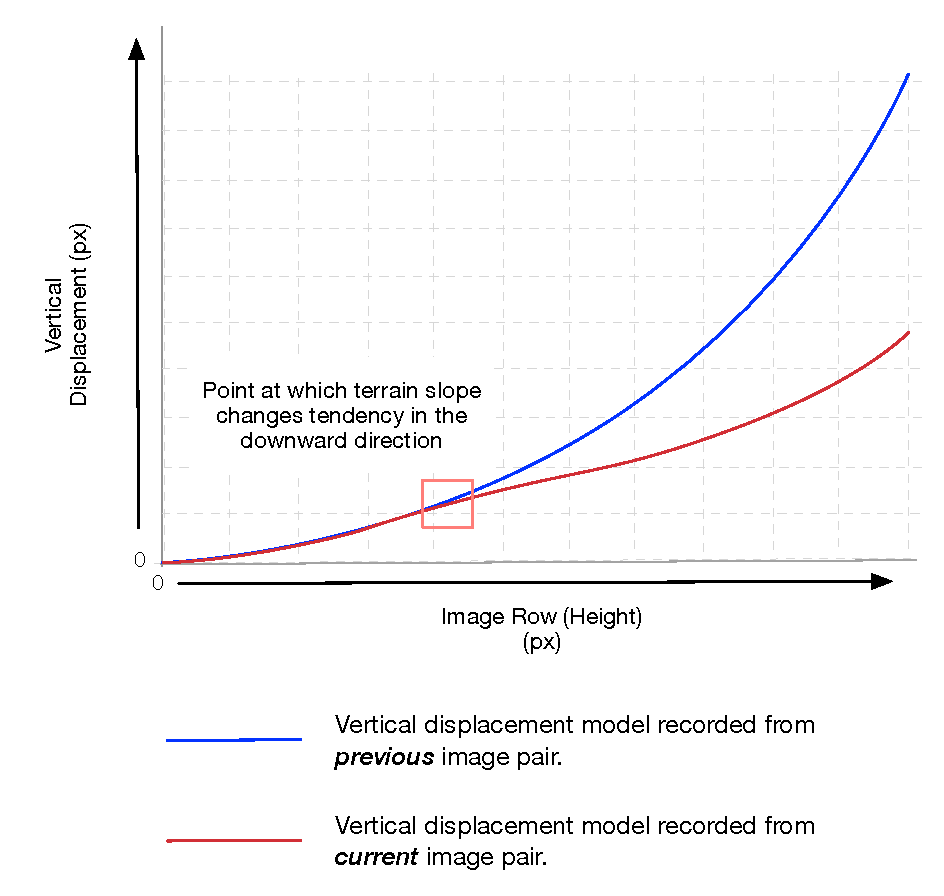
\includegraphics[width=0.9\linewidth]{images/gradient_graph.pdf}
\caption{Simplified example of recorded change in terrain gradient indicating a downwards slope (general reduction in recorded displacement).}
\label{fig:gradient}
\end{minipage}
\end{figure}
 
 % ADD FIGURE SHOWING DIFFERENCE BETWEEN OBSTACLE AND GENERAL CHANGE IN TERRAIN.
 
\subsubsection{Calibration \& Focus of Expansion}
\label{hypo-calib}

When considering the use of input supplied by an optical camera, a crucial aspect lies calibration of the camera lens. The primary requirement for performing calibration stems from the need to identify and correct the \textit{distortion} observed in images that are captured through a \textit{pinhole camera} lens \cite{camera-calib}. 

Failure to correct such distortion can result in significant inaccuracies being observed between the perceived motion of an object captured in an image, and the actual movement that it demonstrates. The effects caused by \textit{perspective distortion} on the perceived motion of objects positioned within the view of a forward-facing camera is a problem that is of particular importance to the success of the approach detailed in Section \ref{hypo-gradient}.

% FIGURE SHOWING PERSPECTIVE DISTORTION.

In the case of many robotic software projects engaging in tasks involving visual navigation or obstacle detection, the calibration of both the camera lens and physical setup allows for future conversion between native camera units (e.g. pixels) and their real world equivalents (e.g. centimetres) \cite{campbell}, \cite{wyeth}. While many computerised solutions to camera calibration do now exist \cite{camera-calib}, all continue to rely upon some form of manual involvement (normally surrounding calibration of the camera lens). 

Through the understanding of a concept known as \textit{Focus of Expansion} (FOE) it was identified that this additional level of complexity associated with camera calibration could instead be replaced with a much simpler approach that focussed exclusively on the analysis of optical flow of features that were contained within a confined ``region-of-interest" located around the horizontal centre of the image.

\begin{wrapfigure}{l}{0.5\textwidth}
\vspace{-20pt}
  \begin{center}
    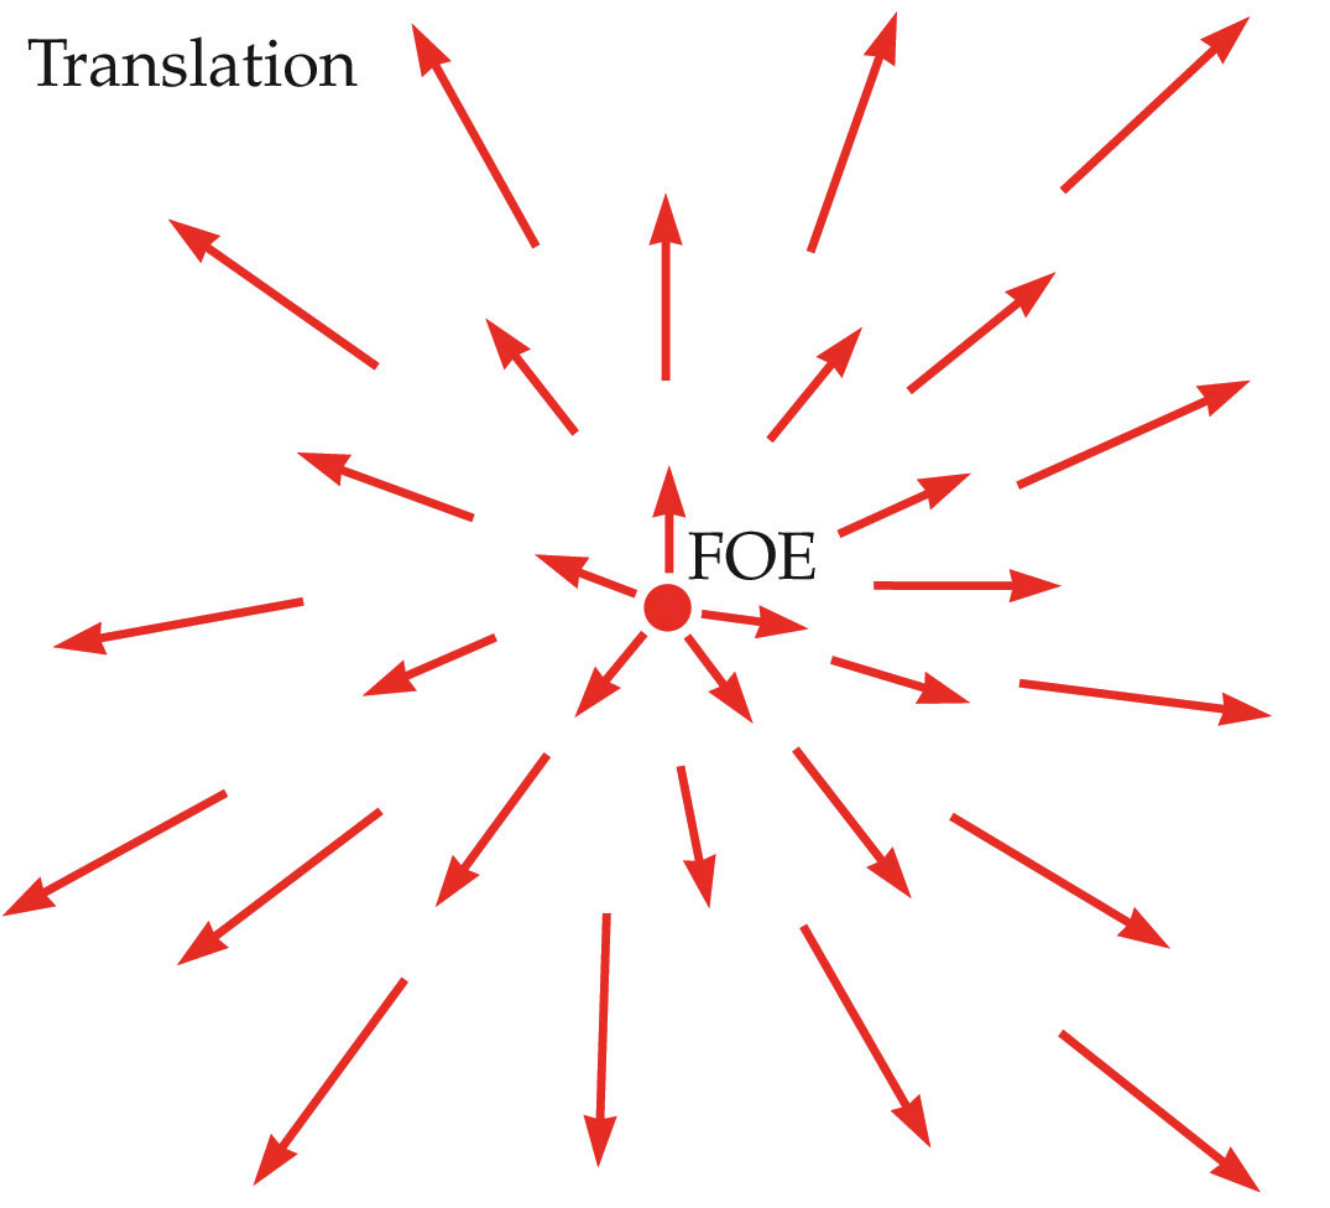
\includegraphics[width=0.45\textwidth]{images/foe.png}
  \end{center}
  \vspace{-10pt}
  \caption{Visualisation of the perceived effects caused by Focus of Expansion. Courtesy \cite{texas-cs}}
  \label{fig:foe}
  \vspace{-20pt}
\end{wrapfigure}

When a camera is moved forward and an image is subsequently taken, all of the motion vectors observed in the resulting perspective image appear to begin from a single point centred along the horizon \cite{stanford-cs}. This `single point' is known as the Focus of Expansion, and acts as the primary metric for an observer wishing to identify the direction in which they are currently headed \cite{texas-cs} (Figure \ref{fig:foe}). 
 
By restricting the tracking of features to only those that lay within a specific range of the FOE, it was hoped that this would allow for a reasonable reduction in the effects caused by perspective distortion without requiring the explicit calibration of camera parameters. 

\subsection{Estimation of Robot Orientation}
\label{hypo-rotation}
An important observation relating to the motion exhibited by a robot, is the notion of it being possible to separate such motion into two main constituent parts; \textit{translation} and \textit{rotation} \cite{campbell}. 

In the context of this project, translation represents the displacement that a robot obtains while travelling along in a single direction. As already discussed in Section \ref{hypo-gradient}, it is currently possible using optical flow analysis, to record translational motion of a forward-moving robot by measuring the level of \textit{vertical displacement} that is demonstrated throughout a series of images captured via a front-facing camera.

The other type of motion that can be demonstrated by a robot is of course, rotation. For a typical mobile robot, rotational movement actually constitutes a change in heading or orientation, which specifically, describes a rotation around the vertical axis \cite{campbell}. In the opposite way to translational movement, changes in rotation can represented by the \textit{horizontal} displacement of features tracked through a collection of images showing the scene in front a robot \cite{labrosse}. 

\begin{wrapfigure}{r}{0.5\textwidth}
\vspace{-20pt}
  \begin{center}
    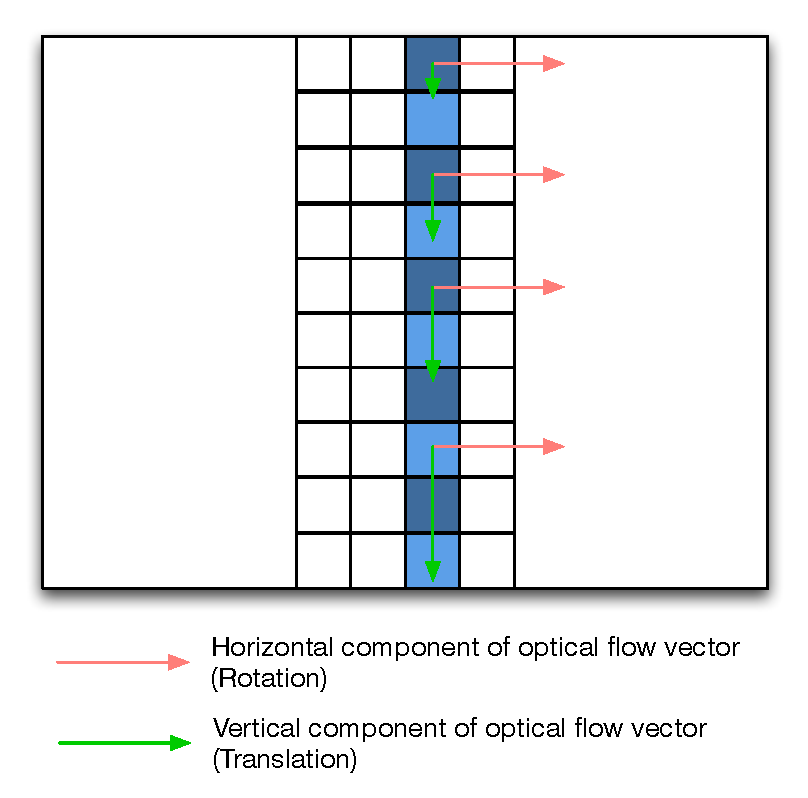
\includegraphics[width=0.49\textwidth]{images/rotation_diag.pdf}
  \end{center}
  \vspace{-10pt}
  \caption{Diagram demonstrating the expected difference in behaviour between the separated vertical and horizontal components of observed optical flow vectors calculated from \textit{forward-turning motion}. Notice that the horizontal-component vectors (i.e. rotation) all share the same magnitude, whereas the vertical-component vectors (i.e. translation) show an increase in displacement travelling towards the bottom of the image.}
  \label{fig:rotation}
  \vspace{-10pt}
\end{wrapfigure}

However, a crucial distinction to be made between these two modes of motion, is the difference observed towards the level of respective displacement that features within an image can demonstrate. In the case of translational motion, features detected towards the top of the image will show a much smaller level of vertical displacement than features located towards the bottom. This is a consequence of the effects caused by motion-parallax, and forms the foundation of the proposal made in Section \ref{hypo-model} for supporting the inference of terrain gradient and obstacle detection. 

In contrast, it is noted that a change in rotation will cause \textit{all} features tracked within an image to move through the \textit{same angle} \cite{campbell} (Figure \ref{fig:rotation}). This is very important, as it subsequently reveals how all of these features should theoretically demonstrate the same level of horizontal displacement regardless of how close or distant they are to the camera at the time of capture.

Taking inspiration from the work of Campbell \textit{et al.} \cite{campbell}, it is predicted that taking the median of these horizontal displacement values will provide an estimation into the change of orientation that a robot has undertaken.

\subsection{Estimation of Robot Speed}
\label{hypo-speed}
For supporting both the inference of terrain gradient conditions and detection of potential obstacles, it is the role of the vertical displacement model (Section \ref{hypo-model})  to provide a delineation of the distance by which tracked features within an image have moved, relative to the position at which they were last detected. 

Using the relationship defined by the standard \textit{speed-distance-time} equation:

\begin{equation}
\text{Speed} = \frac{\text{Distance}}{\text{Time}} 
\end{equation}

it becomes possible to estimate the speed at which the robot the travelling when it is assumed that the time interval between the capture of subsequent images remains constant.

Therefore, a proposed extension to the vertical displacement model would instead see a number of separate models produced during the calibration stage, where each would represent the distance of vertical displacement demonstrated by the terrain as the robot travels at differing speeds (Figure \ref{fig:speed}).

\begin{figure}[ht!]
\centering
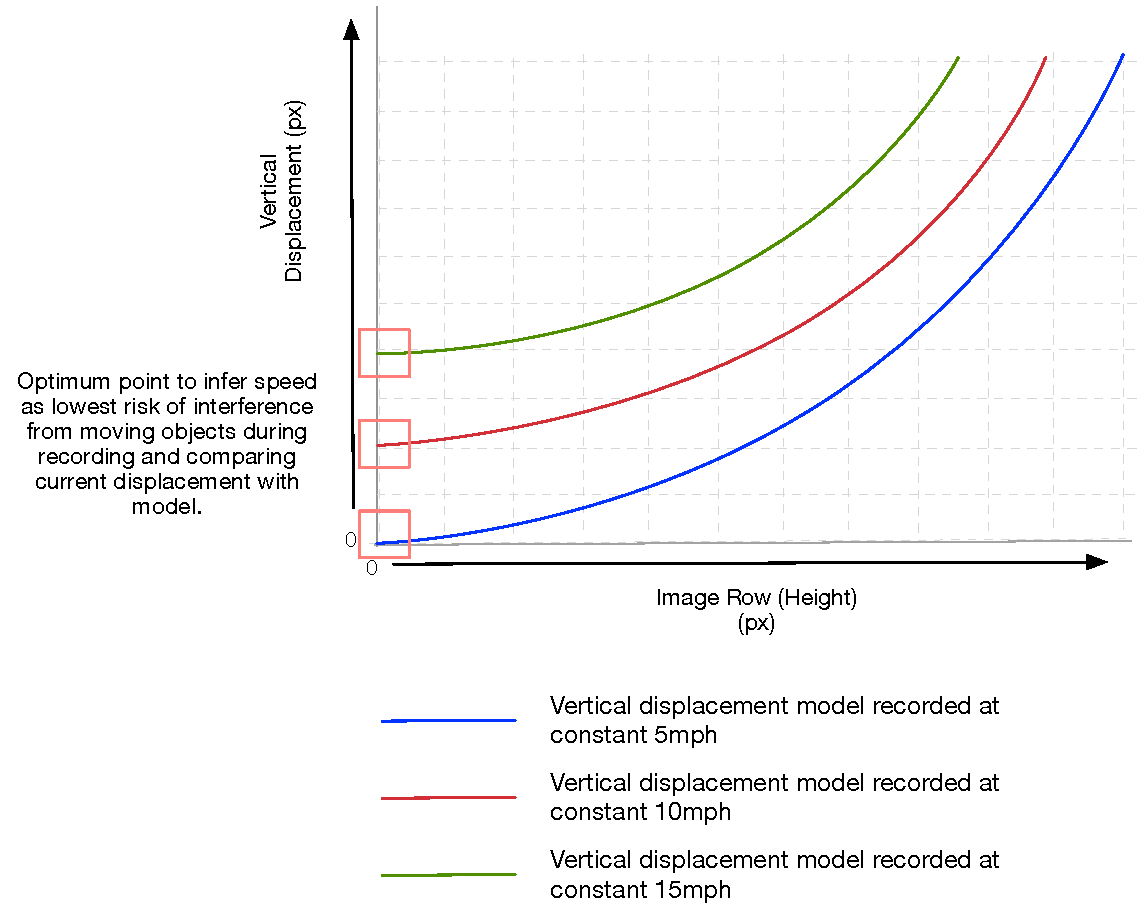
\includegraphics[scale=0.6]{images/speed_graph.pdf}
  \caption{Diagram indicating examples of alternative vertical displacement models calculated while travelling at different constant speeds. To infer the current speed using the calibrated vertical displacement models, the current displacement would be compared with the recorded displacement across each of the alternative displacement models before selecting the model that best fits the current displacement as an indication of the current speed.}
\label{fig:speed}
\end{figure}

Once these multiple models have been established, it would not become an unfeasible task to further enhance the system in order for it to calculate which of the models best matches the current general trend of displacement demonstrated, which therefore would allow for it to present an estimation into current speed of travel.

\section{Analysis}

The main focus for this project falls upon conducting research as part of an investigation into the proposed hypothesis. 

As such, the overall plan for the project intended to perform as much experimentation into the aspects discussed in the hypothesis (see Section \ref{hypo-gradient}) as was feasibly achievable within the three month deadline set for the major project.

\subsection{Breakdown of Research Aims}
\label{aims}

Following the conceptualisation of the working hypothesis, it was necessary to devise a formal list of ``high-level" research aims based upon the proposals that were previously set out. 

Given that these were indeed research-focussed aims, it was expected that they would be completed within a specific sequential order, as this would allow for the work of each subsequent aim to build upon the work of its predecessor.

As there was a relatively high time constraint on the project (with respect to many of the previous projects investigated), it was decided that these aims should be decomposed further into primary and secondary categories.

\subsubsection{Primary Aims}
\label{primary-aims}

The following aims consist of those deemed most important in fulfilling the core motives behind the project investigation. Unsurprisingly, these `primary' aims were also responsible for laying the `groundwork' from which any `secondary' aims could then continue.  

\begin{enumerate}
	\item Establish which out the following appearance-based template matching similarity measures:
		\begin{itemize}
			\item Euclidean Distance
			\item Correlation Coefficient
			\item Histogram Correlation
			\item Histogram Chi-Square
		\end{itemize}
	 best supports the predicted positive correlation between the vertical position of features within an image, and the level of vertical displacement demonstrated (see Section \ref{hypo-model}).
	 \item Implement a means of using the generated model of vertical displacement to identify potential obstacles and changes in terrain gradient based upon the predicted `comparative trend' behaviour detailed in Section \ref{hypo-model}.
\end{enumerate}

\textbf{Note to the Reader:} 

It was deemed important at this point to inform the reader that due to significant issues discovered during experimentation, combined with a lack of author experience and general time constraints, it became progressively clear that work would only be able to focus exclusively on the first primary aim detailed above, before hitting the project deadline. Further discussion regarding this is available as part of the critical evaluation within Chapter 4.

\subsubsection{Secondary Aims}

Additional proposals from the hypothesis that provided further enhancements or abilities were classified as `secondary' aims. While optimistically, it was hoped that such functionality could be implemented in the time available, it was deemed more than likely that such aims would fall outside of the scope of the major project.

\begin{enumerate}
	 \item Further extend the capabilities of the vertical displacement model as discussed in Section \ref{hypo-speed} to provide estimates into the current speed of travel demonstrated by the robot.
	 \item Add support for providing an estimation of the robot's change in orientation using the approach detailed in Section \ref{hypo-rotation}.
\end{enumerate}

\subsection{Breakdown of Experiment Work}

As part of the initial planning stage, expected tasks relating to ``experimental research" were further decomposed into one of four key stages. This was to ensure that there was a full understanding into all of the different kinds of work involved in performing research experiments, which in turn would allow for adequate attention to be given in planning the finer details for each experiment. 

\begin{itemize}
	\item \textbf{Stage One - Data Collection:} In order to evaluate the approaches proposed within the investigation, it would first be necessary to collect and verify image data that could provide an appropriate basis for testing.
	\item \textbf{Stage Two - Setup of Testing Environment:} Prior to beginning any experimentation, it was important to establish a stable and robust testing environment for the evaluation of the implemented methods. In the context of this project, this would include the implementation of an configurable `testing rig' capable of running and evaluating multiple sequences of tests automatically.
	\item \textbf{Stage Three - Establishment of Ground Truth Data:} Compilation of verified results known to represent the ``true" behaviour of the various aspects under investigation. Used as the means of evaluating the relative success of experiments conducted.
	\item \textbf{Stage Four - Implementation of Hypothesised Approaches:} Implementation of the actual approaches and predictions detailed within the proposed working hypothesis (see Section \ref{hypo-gradient}).
	\item \textbf{Stage Five - Evaluation of Experiment Results:} Analysis of the performance results obtained for each of the implemented approaches, focussing in particular on aspects regarding the accuracy of each method when tested against a variety of datasets.
\end{itemize}  

Stages one and two would be performed initially, in order to ensure everything was prepared for the ``bulk" of the investigative work to come within stages three and four. As part of this investigative work, a number of potential appearance-based template matching methods were due to be implemented over a number of working `iterations'. 

Stages three and four would require repeating over every new iteration, each time focussing upon a different method to \textit{implement} and subsequently \textit{test}, before finally moving to stage five in order to conduct an evaluation into the performance of each of the implemented methods.

\subsection{Deliverables}

As is typically the case with research-based projects, it was expected that the majority of deliverables resulting from the completion of tasks would consist mostly of experiment results and evaluation conclusions:

\begin{itemize}
	\item A collection of test images used to evaluate implemented experiments. This may either be images from an existing dataset \cite{ucl-dataset} \cite{baker-dataset}, \cite{mpi-dataset}, or images captured specifically for this project.
	\item A set of predicted experiment results used in evaluating the results obtained from each conducted experiment.
	\item A collection of recorded experiment results, represented as a series of plotted 2D-scatter graphs with the addition of moving averages to allow for the easy identification of expected behaviour trends.
	\item This report, containing information regarding the background to the experiment and hypothesis, details on the experiment methods and a discussion of the results obtained.
 \end{itemize}

However as this project would also focus on producing software (an implicit requirement in the submission as department major project), inevitably there was the expectation of additional deliveries relating to both the development of software and undertaking of project-management:

\begin{itemize}
	\item A series of individual `test rig' applications provided for each primary experiment undertaken.
	\item Accompanying unit and regression tests suites for each separate software module.
	\item Accompanying documentation for produced software.
	\item Breakdown of the current status of remaining work, including details of both ``high-level" and constituent tasks, in addition to details regarding previous project performance (e.g. `burn-down' and `throughput' charts (discussed further in Section \ref{mgmt}).
\end{itemize}

\section{Research Methodology}

This was a project in which the work involved was potentially subject to a great deal of change and re-organisation, arising as a result of attempting to solve a problem that had no fully-defined solution. 

Given this fact, any amount of significant upfront planning and design was deemed unfeasible, as in the most likely of cases, it was expected that a significant proportion of these ``fixed" decisions would eventually undergo some kind of modification following the discovery of issues or better alternatives.

Experiments were instead conducted over a number of project `iterations', in which all of the work associated with a particular experiment would be completed before moving onto the next experiment. This included the design of the experiment itself, the development and testing of associated software, and the gathering and evaluation of result data. 

\subsection{Qualitative \& Quantitative Research}

The project consisted of both qualitative and quantitative research aspects. Qualitative research focussed on providing the outline to the proposed hypothesis \cite{research-types}, aiming to investigate the reasons behind \textit{why} it was possible to use visual stimuli in aid of detecting potential hazards and changes in gradient across the observed terrain. This kind of research was conducted early within the project timeline and took the form of reading existing papers and examples of previous visual-based projects relating to the topics identified for this project.

Quantitative research involved the gathering and subsequent analysis of data in order to try and identify \textit{how} various approaches could be used to solve the question topics uncovered within the qualitative research (i.e. the hypothesis) \cite{research-types}. In the context of this project, all of the experiments discussed in Chapter 2 fell under the category of quantitive, rather than qualitative research.

\subsection{Management Process}
\label{mgmt}

Traditional, plan-driven approaches towards software development tend to expect all requirements are gathered up front prior to beginning any planning, design or implementation. For this project, such an approach would have been unsuitable, as it was likely that ``requirements" would be created, modified and removed much later into the project as a result of recent discoveries in the successes and failures of previous experiments. 

Instead, the decision was taken to adopt a SCRUM-based methodology for the planning, recording and organisation of tasks, work would be partitioned into a series of time-boxed releases and subsequent sprints. By following an agile methodology process, development work could begin  more quickly, and in conjunction with ongoing research and experiment evaluation. Through choosing to begin building working software early, even with limited functionality, it would become possible to potentially contribute some of this work back into ongoing research (e.g. use of the same testing rig ``shell" within a new experiment) and in turn improve the overall efficiency.

As the SCRUM methodology is founded upon empiricism \cite{scrum}, this allows it to appreciate that unpredicted changes cannot effectively be addressed using a plan-driven approach. The work conducted for each iteration was prioritised based upon discussions with the project supervisor. New work items were added to a list of outstanding tasks (product backlog), before being organised into a specific collection of tasks (sprint backlog) scheduled for completion within a particular sprint.

Each sprint followed a ``five-day on, two-day off" development cycle, which provided a buffer to help in situations where work took significantly longer than expected. Sprint planning meetings were arranged for the same time as the weekly group project meeting, allowing for planning of work for the coming week, along with the opportunity to discuss changes that either party felt were required in light of new experiment results.

In terms of tracking project progress, feedback for sprints and releases was provided via a combination of burn-down and throughput charts (see Appendix C - Figures \ref{fig:burndown} and \ref{fig:throughput}), that were created using the \textit{Burndown.io}\footnote{\url{http://burndown.io/#cgddrd/cs39440-major-project}} and \textit{Waffle.io}\footnote{\url{https://waffle.io/cgddrd/cs39440-major-project}} web services. 

While both provided graphical representation of work completed, throughput charts focussed on comparing the frequency of completed tasks over a fixed range of weeks, whereas burn-down charts plotted the amount of outstanding work within an individual sprint or release, in relation to the time that was left before it closed.

\begin{figure}[ht!]
\centering
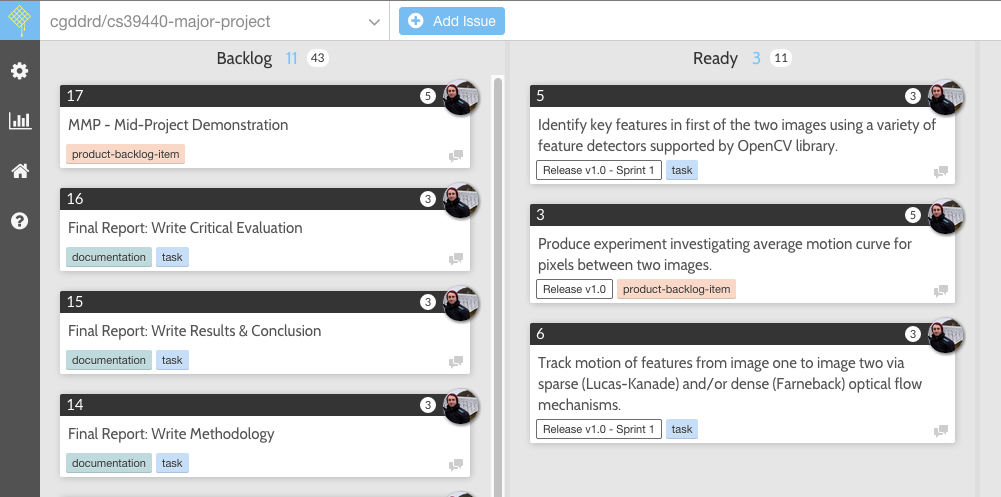
\includegraphics[scale=0.3]{images/kanban.png}
  \caption{Day-to-day tasks were managed via the use of web-based KANBAN-style interface (Waffle.io\footnote{\url{https://waffle.io/cgddrd/cs39440-major-project}}), that connected directly to the project Github account where all of the SCRUM backlogs were stored.}
\label{fig:kanban}
\end{figure}

%\subsection{Testing \& Evaluation of Experiments}
%
%In evaluating the performance of experiments, it was not simply the case that results would equate to a clearcut pass or fail. Instead, testing was a ``subjective" task, involving the use of previously established ground truth data that an experiment would subsequently be expected to replicate as closely as possible. 
%
%The performance of each method tested within an individual experiment would be assessed by comparing how closely each of the recorded results matched the results predicted. 





